\documentclass[a4paper,12pt]{article}

\author{\textbf{Софиа Белен Лопес Висенс}\\
    Группа Б02-903\\ 
\large Московский физико-технический институт}
\title{\textbf{Задание 2}\\
Молекурялная динамика}
\date{}

\usepackage[margin=0.9in]{geometry}
\usepackage{graphicx}
\usepackage{float}
\usepackage[utf8]{inputenc}
\usepackage[T2A]{fontenc}
\usepackage{textcomp}
\usepackage{amsmath, amssymb}
\usepackage{siunitx}
\usepackage{subcaption}
\usepackage{multirow}
\usepackage{xcolor}

\definecolor{grey}{HTML}{ba000f}
\definecolor{red}{HTML}{990505}
\definecolor{green}{HTML}{2e8a07}

\renewcommand{\figurename}{Рис.}
\renewcommand{\tablename}{Таблица}
\renewcommand*\contentsname{Содержание}

\begin{document}
\maketitle
\newpage
\tableofcontents
\newpage

\section{Радиальная функция распределения}

\begin{figure}[H]
    \centering
    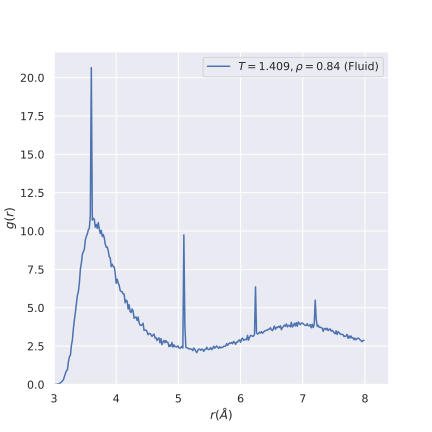
\includegraphics[width=0.8\textwidth]{../../media/rdfYarnell.pdf}
\caption{Радиальная функция распределения для жидкого Аргона
при \(\rho = 0.0213 \frac{atoms}{\si{\angstrom}^3}\), 
\(T = 85^\circ K\). Соответственные параметры в единицах
Леннарда-Джонса \(\rho = 0.84\), \(T = 1.409\).}
\end{figure}

\section{Автокорреляционная функция скорости}

\begin{figure}[H]
    \centering
    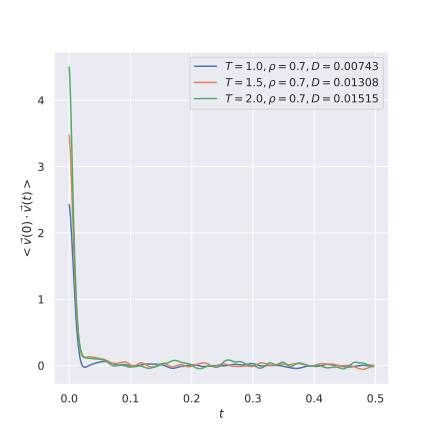
\includegraphics[width=0.8\textwidth]{../../media/vac.pdf}
\caption{График автокорреляционной функции
    скорости в зависимости от времени при различных
температурах. Расчёт коэффициент самодиффузии с
помощью формулы Грина-Кубо.}
\end{figure}

\section{Расчёт коэффициента самодиффузии}

{\color{red} Maybe we are still in subdiffusive regime?}

\begin{figure}[H]
    \centering
    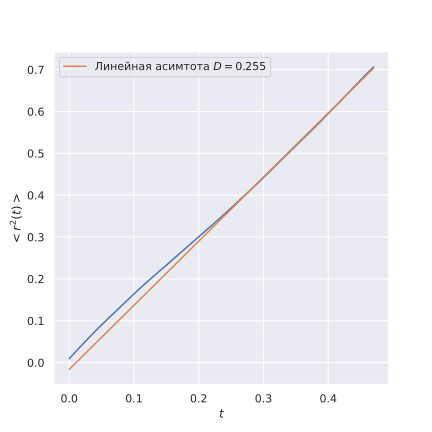
\includegraphics[width=0.8\textwidth]{../../media/diffusion.pdf}
\caption{График зависимость среднего квадратичного
смещения в зависимости от времени. Расчет коэффициента
самодиффузии через формулу Эйнштейна-Смолуховского.}
\end{figure}

\begin{table}[H]
    \centering
    \caption{Коэффициент самодиффузии полученный через
    формулу Эйнштейна-Смолуховского и Грина-Кубо при 
\(\rho = 0.7\).}
    \label{tab:label}
    \begin{tabular}{|c | c | c | c |}
        \hline
        Темература & Эйнштейна-Смолуховского & Грина-Кубо 
                   & Ожидаемое значение\\
        \hline
        \hline
        1.0 & 0.092 & 0.00743 & {\color{red}0.105} \\
        1.5 & 0.119 & 0.01308 & {\color{red}0.156} \\
        2.0 & 0.153 & 0.01515 & {\color{red}0.217} \\
        \hline
    \end{tabular}
\end{table}

\section{Сравнение с первым заданием}

{\color{red} Вопрос: Как это \(<\Delta r^2(t)>\)
связано с значением из другого пункта?}

\begin{figure}[H]
    \centering
    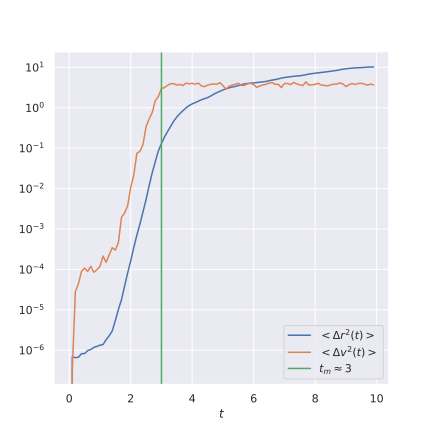
\includegraphics[width=0.8\textwidth]{../../media/tm.pdf}
\caption{Усреднённые разбегания координат \(<\Delta r^2(t)>\) 
и скоростей \(<\Delta v^2(t)>\) на двух траекториях,
рассчитанных из тождественных начальных условий с 
шагами \(\Delta t_1 = 0.001\) и \(\Delta t_2 = 0.0001\).
При температуре \(T = 1.0\) и плотности 
\(\rho = 0.7\) получаем коэффициент
самодиффузии \(D = 0.079\). Он оказывается на порядок
меньше значения полученного с помощью соотношения
Эйнштейна-Смолуховского но сравнимый с значением из
метода Грина-Кубо.}
\end{figure}

\section{Влияние термостата на расчет коэффициента диффузии}

\begin{figure}[H]
    \centering
    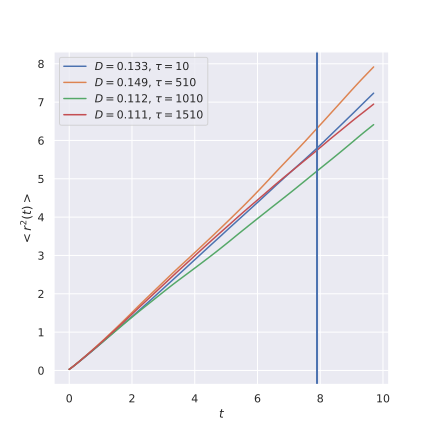
\includegraphics[width=0.8\textwidth]{../../media/thermostat.pdf}
\caption{График зависимость среднего квадратичного
смещения в зависимости от времени. Расчет коэффициента
самодиффузии через формулу Эйнштейна-Смолуховского при
температуре \(T = 1.5\) для различных характерных 
величин термостата \(\tau\).
Вертикальная линия показывает момент, начиная с которого 
мы рассчитаем коэффициент диффузии.}
\end{figure}

\section{Сравнение с результатами Naghizadeh и Rice}

Для жидкостей \(Ar\), \(Kr\), \(Xe\) и \(CH_4\), 
описываемых потенциалом Леннарда-Джонса,
Naghizadeh и Rice экспериментально получили следующую 
зависимость коэффициента самодиффузии \(D\)
при \(T < 1.0\), \(P < 3.0\):

\[
    log_{10} D = 0.05 + 0.07 
    P - \frac{1.04 + 0.1 P}{T}.
\] 

\begin{table}[H]
    \centering
    \caption{Сравнение значений \(\log_{10} D\)
        полученное соотношением Naghizadeh и Rice с
        значениями, полученными путём моделирования.
    \(<|\Delta|> = 1.011\).}
    \begin{tabular}{| c | c| c | c | c| }
        \hline
        \(T\) & \(P\) &\(\log_{10} D\),  Моделирование & 
        \(\log_{10} D\), Эксперимент &
        \(|\Delta|\)\\
        \hline
        0.20 & 0.13 & -2.69 & -5.21 & 2.52 \\
        0.25 & 0.27 & -2.65 & -4.20 & 1.55 \\
        0.30 & 0.42 & -2.61 & -3.53 & 0.92 \\
        0.40 & 0.71 & -2.44 & -2.68 & 0.24 \\
        0.50 & 1.01 & -2.51 & -2.16 & 0.35 \\
        0.60 & 1.35 & -2.45 & -1.81 & 0.64 \\
        0.70 & 1.62 & -2.39 & -1.55 & 0.84 \\
        0.75 & 1.78 & -2.33 & -1.45 & 0.88 \\
        0.80 & 1.93 & -2.44 & -1.36 & 1.08 \\
        0.90 & 2.27 & -2.29 & -1.20 & 1.09 \\
        \hline
    \end{tabular}
\end{table}

\end{document}
